\documentclass[12pt]{book}
				%这里是导言区

\usepackage{ctex}
\usepackage{amsmath}
\usepackage{graphicx}
\usepackage{url}
\usepackage{listings}
\usepackage{cite}
\usepackage{subfigure}
\usepackage{caption}
\usepackage{exscale}
\usepackage{relsize}
% \setmainfont{Caladea}

\lstset{
	frame=shadowbox,
	xleftmargin=2em,
	xrightmargin=2em,
	aboveskip=1em,
	numberstyle=\tiny,
	basicstyle={\ttfamily}
}

\setlength{\oddsidemargin}{0mm}
\setlength{\evensidemargin}{0mm}
\usepackage[left=25mm,right=20mm,top=25mm,bottom=20mm]{geometry}

\linespread{1.25}

\title{基于奇异值变换的航空图像增强}
\author{王佳欣}
\date{2018年5月}

\begin{document}
	\maketitle	 	
	%标题、作者、日期 按照预定的格式展现出来
	\tableofcontents


	\chapter{绪论}
		\section{航空图像增强概述}随着航空技术及无人机技术的快速发展,航拍图像成为了现今获取地面观察数据的重要来源。航拍图像在气象观测、国土调查、疫情控制、地理测绘等领域起重大作用。由于环境污染加重以及恶劣天气的存在,社会对航空图像的质量提出了更高的要求。例如,在沙尘、雾霾等天气条件下,图像采集设备难以获得清晰图像以便后续工作的开展。因此开展对航空图像的增强话处理意义重大。%\\ \indent
		
本课题针对模糊不清、对比度低的灰度航空图像,提出了基于奇异值分解和二维离散小波变换的图像增强处理。并通过主观评价和诸如平均值、标准差、直方图的客观评价指标进行评价。.
		\section{航空图像}
			\subsection{航空图像特点}航空照片是从空中飞机上获取的特定景观或地理特征的图像,或者是从地面以上给定距离指向地球的传感器的图像。 根据他们拍摄的时间以及拍摄角度的不同,可以制作一些其他方式无法具备的具有大量信息的图片。 很多时候,从不同的角度拍摄航拍照片有助于建立准确的地图。由于人类摄影无法处理的角度和距离,航拍也对电影业非常有用。 在军事方面,航拍照片用于监视敌人的线路和间谍活动,而占星家依靠它拍摄地球和相关机构的照片。使用航拍照片可以获得立体视图,可以感受到三个维度:长度、宽度和高度,而不同于其他图片只能感知二维信息。通过查看照片可以估计地面上的物体几何特征。 虽然人眼在观看某一物体时的分辨率有限,但航空相机却没有。 航空相机比人眼对更多的光波和辐射敏感; 因此航空图像可以提供各种物体之间的相对间距和距离。

任何物体都有不同的电磁波反射和辐射特征,遥感技术是利用飞机等飞行器或者人造卫星对反射和辐射特征进行采集和分析,探测、分析和识别特定对象的技术。根据采集平台分类,遥感可以分为地面遥感、航空遥感和航天遥感;根据电磁波波长分类,遥感可分为微波遥感、红外遥感和可见光近红外遥感。由于航空遥感具有机动灵活且免受云层干扰等诸多优点,因此本文中所有的实验数据都采用“航空遥感图像”(简称为“航空图像”),更具体地,本研究中所说的航空图像指在飞机上拍摄的航拍图像,航拍图像有以下优点\cite{?}:
				\begin{itemize}
					\item \emph{航空图像信息容量大,空间分辨率大。}
					\item \emph{航拍图像应用灵活。可灵活的设置图像分辨率以及采集频率等信息,另航空图像在空间以及时间上具有较强的灵活性,有利于制定合适的方案。}
					\item \emph{航空图像信息的获取方便。}
				\end{itemize}

			 但是航拍图像也有受环境信息干扰大、勘探范围有一定的局限性的缺陷。
			\subsection{图像增强的意义}图像增强作为图像处理的一个古老而重要的分支,在不断地应用需求变化面前,也在不断更新其研究目标和发展其增强处理方法技术。通常,由于场景本身所包含的动态范围、光照条件、图像捕获设备如数码相机的局限,以及摄影者本身的技术问题等多种因素影响,多数情况下,会使得拍摄的图像达不到人们预期的目标,如场景中的运动目标产生的运动模糊、由于曝光不恰当引起的场景细节损失或是弱小目标辨识不清等,都会对后期的图像前后景分割、目标识别、目标跟踪和最终的图像理解以及预测分析等带来困难。而图像增强本身的目标就是为了突出图中感兴趣的区域、降低或去除不需要的图像信息,以此来加强和获取用户觉得有用的信息,进而得到更加适合于人/机器对图像进行理解和分析处理的表现形式或是富含更多细节信息的图像的相应处理方法\cite{?}。

图像增强基本上提高了人类对图像信息的可解读性或感知能力,并为其他自动图像处理技术提供了更好的预处理。图像增强的主要目的是修改图像的属性,使其更适合于给定的任务和特定的观察者。在此过程中,图像的一个或多个属性被修改。属性的选择和修改的方式是特定于特定任务的。此外,由于观察者的特殊因素,如人类视觉系统,将在图像增强方法的选择中引入大量的主观性。有许多技术可以在不损坏数字图像的情况下增强数字图像。图像增强分为空域图像增强和频域图像增强:

在空域图像增强技术中,我们直接处理图像像素。 操纵像素值以实现期望的增强。 在频域方法中,图像首先被转换到频域,即首先计算图像的傅里叶变换。所有的增强操作都是在图像的傅里叶上执行的,然后执行逆傅里叶变换以得到最终的图像。 执行这些增强操作是为了修改图像亮度,对比度或灰度级的分布。 结果,输出图像的像素值(强度)将根据应用于输入值的变换函数进行修改。图像增强应用于图像应该被应用和分析的每个领域。 例如,医学图像分析,卫星图像分析等。

图像处理算法提供了多种方法来改进原始图像以获得视觉上可接受的图像。根据特定任务,图像内容,观察者特征和观看条件的需求来选择这些图像增强技术。点处理方法是最原始的。对于黑暗的图像,灰度级的扩展是通过使用分数指数的幂律变换完成的。对数转换对于增强图像较暗区域中的细节非常有用,但牺牲了较亮区域中较高级别值的细节。图像的直方图能提供重要信息是关于图像的对比度。直方图均衡是通过均匀重新分配灰度值来扩展对比度的变换。只有全局直方图均衡可以简单地自动完成。
		%	\subsection{国内外研究现状}王志伟\cite{?}运用基于尺度变换和幂次变换的Retinex方法研究了模糊不清的航空图像的图像增强和道路提取,并在算法中考虑了景深信息,该算法成功使模糊不清的航空图像的的完善,为后续的道路提取打下了坚定的基础。
			
			\section{本文主要内容与结构}本文以航空图像为研究对象,分析了航空图像的特点和图像增强的一般方法和意义,就目前适用于航空图像增强领域的常用算法展开研究,并通过实验证明本文所提出的方法的有效性。本论文主要研究内容如下:

$(1)$探究航空图像相较于其他图像的优势和其在具体的应用中受何限制。进一步探究航空图像在特定情况下的缺陷,介绍一些增强算法,使这些缺陷得到进一步的消除以便进行后续处理以及观察。

$(2)$研究常用的图像增强处理算法,分析这些方法各种航天图像增强上的效果,例举其优点及其缺点,并于本文提出的方法进行比较。

本文的具体结构安排如下:

第一章,介绍本课题的研究背景和意义,分析了航空图像的特点及其图像增强的意义,并简单介绍了一下图像增强的一般算法。

第二章,介绍了常用的图像增强方法直方图均衡算法以及Retinex增强算法。探究了直方图均衡在低对比度图像上的显著增强效果以及其在在增强的同时也模糊了细节的缺陷。并阐述了基于人眼视觉特性和颜色恒常理论的Retinex增强算法在航空图像上去雾应用上的显著特点。

第三章,介绍了本文算法DWT-SVD增强算法,详细介绍了奇异值分解算法和离散小波变换在图象上的应用以及两者的组合在图像增强上的优点。

第四章,介绍图像评价的几个指标客观指标和主观指标,并将几个算法的结果图进行比较,以及结果图的客观指标进行比较。

	\chapter{常用的图像增强方法}本章首先介绍直方图均衡增强算法和Retinex增强算法的基本原理和发展历程,阐述他们在航空图像增强中的应用。	
		\section{直方图均衡}
			\subsection{直方图均衡增强算法理论}直方图均衡通常会增加许多图像的全局对比度,特别是当图像的可用数据由近似对比值表示时。通过这种调整,直方图上的强度可以更好地分布,使局部对比度较低的区域获得较高的对比度。直方图均衡通过有效地分散最频繁的强度值来实现这一点。该方法在背景和前景都很亮或两者都暗的图像中很有用。例如,该方法可以更好地观察X射线图像中的骨骼结构,并可以更好地了解曝光过度或曝光不足的照片的细节。该方法的一个关键优点是它是一种相当直接的技术和可逆运算符。所以理论上,如果直方图均衡函数是已知的,那么原始直方图可以被恢复。该方法的一个缺点它可能增加背景噪声的对比度,同时减少可用信息。

直方图均衡算法的改进是使用多个直方图(称为子图)来强调局部对比度,而不是整体对比度。直方图均衡改进算法包括自适应直方图均衡化,对比限制自适应直方图均衡化,多峰直方图均衡化和多用途$\beta$优化生物统计图均衡化。这些方法的目标,是通过改进HE算法来改善对比度而不产生亮度均值偏移和细节损失伪影。直方图均衡化的信号变换也在生物神经网络有所应用,作为输入统计量的函数使神经元的输出发放速率最大化。
直方图均衡是一般的直方图重新映射方法的一个特例。这些方法试图调整图像以使其更容易分析或改善视觉质量,例如Retinex。
			\subsection{直方图均衡增强算法实现}直方图描述了一幅图像的绘图统计信息,是一个关于灰度的函数,如令$x$表示灰度值,则离散函数$f(x)$表示当$x$为特定灰度值时,一幅图像上灰度值为$x$的像素的数量。

直方图均衡属于图像增强技术中的空域方法,即直接对像素值施加以相应的操作以获得增强效果。直方均衡是一种利用图像的直方图像来调整图像对比度的一项技术,该技术基于将原场景图像的直方图经重新映射后得到一个接近于均匀分布的概率密度函数的新的直方图的思想,是一种简单有效的对比度拉伸技术\cite{?}。	

直方图均衡的目的是使原始图像原有的灰度分布即直方图,重新在一定的范围内“均匀”分布。而对于原始图像直方图具有的谷值和峰值,直方图均衡处理后仍具有原来的形状,并且变得平滑。以下将阐述直方图均衡的数学表达。

考虑连续的灰度值,用r表示原始出翔的灰度。假设r的取值区间是$[0,L-1]$,灰度值变换公式为
\begin{equation}s=T(r),0 \leq r\leq L-1 \end{equation}
%\begin{eqnarray*}
%x^n+y^n &=& z^n \\
%x+y &=& z
%\end{eqnarray*}
%其中两个&号之间的是公式间对齐的位置,用\\隔开各行公式。上面输出的公式是没有编号的,如果需要自动编号,可以将eqnarray*改为eqnarray 。 

灰度变换公式满足以下条件
			\begin{itemize}
				\item \emph{$T(r)$在区间$0\leq r\leq L-1$上为单调递增函数。}
				\item \emph{当$0\leq r\leq L-1$时,$0\leq T(r) \leq L-1$。}
			\end{itemize}

原始图像的灰度值可视为$[0,L-1]$内的随机变量。用概率密度函数(probability density function,PDF)来描述这些随机变量。有如下公式:
\begin{equation}p_s(s)=p_r(r)|\frac{dr}{ds}|\end{equation}	
其中$p_r(r)$表示随机变量$r$的概率密度函数,$p_s(s)$表示随机变量$s$的概率密度函数。并有如下公式:
\begin{equation}     s=T(r)=(L-1)\int_0^r p_r(v)\,dv    \end{equation}	
\begin{equation}     \frac{ds}{dr}=\frac{dT(r)}{dr}=(L-1)\frac{d}{dr}\left[\int_0^r p_r(v)\,dv 	\right]=(L-1)P_r(r)     \end{equation}
\begin{equation}     p_s(s)=p_r(r) \left| \frac{dr}{ds}\right| =p_r(r) \left| \frac{1}{(L-1)p_r(r)} \right| = \frac{1}{L-1},0 \leq s \leq L-1    \end{equation}
其中,v是积分假变量。公式的右边是随机变量$r$的累计分布函数(cumulative distribution function, CDF)。由公式$(2.5)$得知得到的$p_s(s)$始终是均匀的,与$P_r(r)$无关。简单的来说就是使原始图像的灰度直方图的累计分布函数均匀分布使得原始图像的对比度变高。以下是一个直方图均衡的例子:
			\begin{figure}[!ht]\centering
				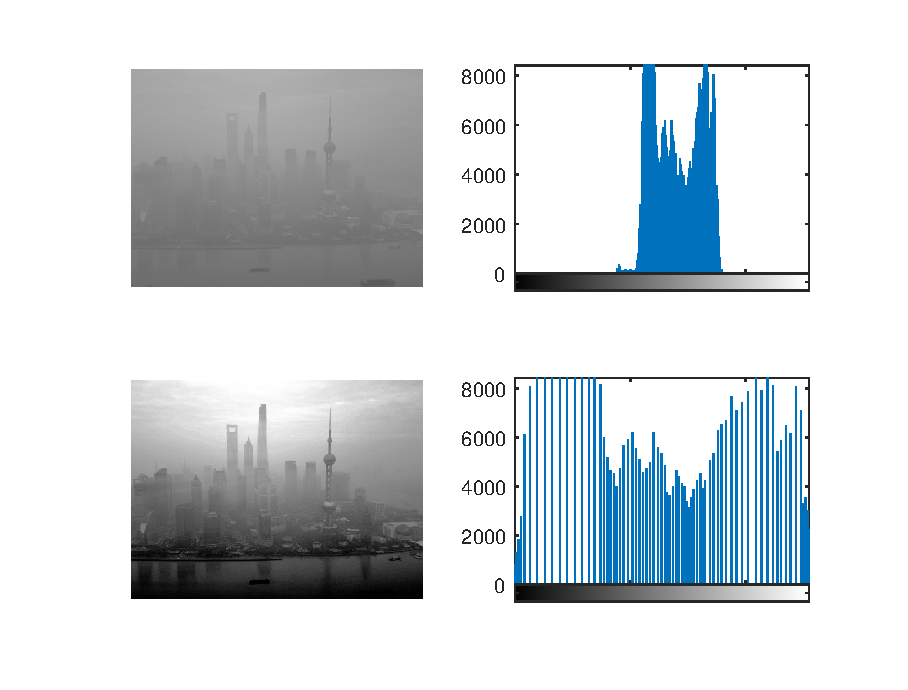
\includegraphics[totalheight=60mm]{./figures/histogramExample.eps}
				\caption{直方图均衡\label{histogram}}
			\end{figure}
从上图可以看出原本对比度很低,模糊不清的原始图像经过直方图均衡后变得更为清晰,视觉效果好。其中,均衡化后图像的灰度直方图形状与原图的灰度直方图相似,只不过被“拉伸"了。直方图均衡有助于图像的增强,但是也有过增强和细节变得更加模糊的缺点。

虽然直方图均衡化后的效果比原始图像好,但是所得的图像在一些轮廓和细节方面处理是不如其他常用的增强算法的,会产生轮廓的模糊等现象。
		\section{Retinex增强算法}	Retinex(Retina-Cortex)理论是在1977年由Edwin Land提出的关于图像增强的理论,器阐述了人通过亮度感知捕捉色度图像在不同亮暗情况下辨认物体的能力。是研究人员模仿人类视觉系统而发展而成的算法,从单尺度Retinex(Single Scale Retinex,ssr)算法改进成多尺度加权平均的Retinex算法(Multi Scale Retinex,msr),再发展成彩色恢复多尺度Retinex算法。由于人眼对亮度、饱和度、对比度拥有相当的分辨能力,基于肉眼视觉感受的航空图像增强有助于观察者分析并且观察航空图像,并从中获取预期的信息和得到预期的视觉效果。Retinex理论包含两个方面的内容:$(1)$物体的色彩具有一致性,不受光的非均匀性的影响。$(2)$物体的颜色不是取决于反射光的强度的绝对值,而是取决于物体对各种波长的发射能力决定的。

Retinex理论通常广泛在可见光图像增强领域有所应用,而航空图像正好可以运用Retinex理论进行分析和处理。一下将介绍有关颜色视觉理论和肉眼视觉的特性的相关知识。
			\subsection{颜色视觉理论和人眼视觉特性}
				\subsubsection{人眼视觉特性}眼睛是一个接受神经系统以及大脑调节和控制的一个复杂光学系统。在长期的生物进化过程中,人类形成了独有的视觉特性,以便适应自然环境以及加强对物体的感知。眼睛的视觉特性有以下几个特点:
				\begin{itemize}
					\item \emph{波长位于$400~800nm$的电磁波是人的眼睛可以看见的电磁波,在这范围内的电磁波也可被称为白光。七色光就是白光通过三棱镜折射而成的。}
					\item \emph{人的眼睛对不同波段的可见光的敏感程度是不一样的,其中对于黄绿光所在波段的电磁波的敏感度较高,而对红蓝光所在波段的电磁波的敏感度较低。}
					\item \emph{人的眼睛对亮度和光强的响应不是线性的。只有光强到一定的阈值时,人的眼睛才能感知光强的变化,并且在黑暗环境下人的眼睛对于光强和亮度的变化比明亮环境下的更敏感。}
					\item \emph{人的眼睛对与细节的分辨能力是有限的。比如,当移动的目标速度变快时,肉眼分辨率下降。}
					\item \emph{对目标亮度和色彩的感知与背景相关。}
				\end{itemize}

通过研究人的眼睛的视觉特性有助于建立相对应的视觉模型,如黑白模型,彩色视觉模式等视觉模型。这些视觉模型的建立应用于图像增强领域以帮助提高人对图像的视觉能力,增强分辨力。
				\subsubsection{颜色视觉理论}彩色视觉色觉是有机体或机器基于其反射、发射或传播的光的波长(或频率)区分物体的能力。 颜色可以通过各种方式进行测量和量化; 事实上,一个人对色彩的感知是一个主观过程,大脑响应当入射光与眼睛中几种类型的视锥细胞反应时产生的刺激。 实质上,不同的人以不同的方式看到相同的照明物体或光源。

色彩视觉的两个互补理论是三色理论和对手过程理论。 Thomas Young和Hermann von Helmholtz在19世纪提出的三色理论或Young-Helmholtz理论指出,视网膜的三种类型的视锥优先对蓝色,绿色和红色敏感。 Ewald Hering在1872年提出了对手过程理论。 它指出,视觉系统以对立的方式解释颜色:红色与绿色,蓝色与黄色,黑色与白色。 这两种理论现在都被认为是有效的,描述了视觉生理学的不同阶段。
光的波长范围以不同程度刺激这些受体类型中的其中一种。例如,黄绿色的光线同样强烈地刺激L和M锥体,但仅仅弱地刺激S锥体。另一方面,红光刺激L锥体比M锥体多得多,而S锥体几乎不刺激;蓝绿光与L锥相比更能刺激M锥,S锥更强烈,也是棒状细胞的高峰兴奋剂;蓝光比红光或绿光更强烈地刺激S锥,但L和M锥更弱。大脑结合了来自每种类型受体的信息,从而产生对不同波长光的不同感知。

存在于L和M视锥中的视蛋白(光敏色素)在X染色体上编码;这些缺陷编码导致两种最常见的色盲形式。编码L型视蛋白中的视蛋白的OPN1LW基因具有高度多态性。很小比例的女性可能有一种额外类型的彩色受体,因为它们在每个X染色体上具有用于L视蛋白基因的不同等位基因。 X染色体失活意味着虽然在每个视锥细胞中仅表达一种视蛋白,但这两种类型都是整体出现的,并且一些女性可能因此显示一定程度的四色视觉[10]。在编码以M个锥体表达的视蛋白的OPN1MW中的变异似乎很少,观察到的变体对光谱灵敏度没有影响。

通过初始颜色对手机制,颜色处理在视觉系统中(甚至在视网膜内)以非常早的水平开始。因此,亥姆霍兹的三色理论和霍林的反对过程理论都是正确的,但三色性在受体水平上出现,并且对立过程出现在视网膜神经节细胞及其以外的水平。在Hering的理论中,对手机制指的是红绿,蓝黄和明暗的相反颜色效应。然而,在视觉系统中,反对的是不同受体类型的活性。一些侏儒视网膜神经节细胞反对L和M锥体活动,其对应于松散的红绿对称性,但实际上沿着从蓝绿色到品红色的轴线延伸。小双分子视网膜神经节细胞反对从S锥体输入来自L和M锥体的输入。这通常被认为对应于蓝黄色的对数,但实际上沿着从黄绿色到紫色的颜色轴。

颜色恒常性是主观恒定性的一个例子,是人类色彩感知系统的一个特征,它确保在变化的照明条件下物体的感知颜色保持相对恒定。 例如,当主要照明为白色阳光时,以及在日落时主要照明为红色时,例如一个青苹果在中午看起来为绿色。 这有助于我们识别物体。

				\subsection{单尺度Retinex}单尺度Retinex算法是在色彩恒常性基础上,经过人眼模拟获得图像的信息的过程,图像模型转化为场景反射和光照分布两个过程。具体流程和算法图下所示:

一幅给定图像$s(x,y)$可以分解为两个不同的图像:反射图像$r(x,y)$和亮度图像$L$,原理图如下:
			\begin{figure}[!ht]\centering
				\includegraphics[totalheight=60mm]{./figures/retinexSSR.png}
				\caption{SSR原理图\label{SSR}}
			\end{figure}

如上图所示,入射光照射在反射物体上,通过反射物体的反射形成反射光进入人眼,得到人所见到的图像,用公式表达为:
\begin{equation}     S(x,y)=R(x,y)L(x,y)    \end{equation}	
其中,$L(x,y)$表示入射图像,他决定了图像中像素多能达到的动态范围,$R(x,y)$表示物体的反射性质图像,即图像的内在属性,$S(x,y)$表示人眼所能接收到的反射光图像。该理论的基本思想是在原始图像中,通过某种方法降低或去除入射图像的影响,从而尽可能保留物体本质的反射属性图像。其一般处理过程如下所示:
			\begin{figure}[!ht]\centering
				\includegraphics[totalheight=30mm,width=160mm]{./figures/retinexSSR1.png}
				\caption{SSR原理图(这个图像要改)\label{SSR}}
			\end{figure}

我们把照射图像假设为空间平滑图像,可得单尺度Retinex算法公式为:
\begin{equation}     r(x,y)=logR(x,y)=log \frac{S(x,y)}{L(x,y)}    \end{equation}
\begin{equation}     r(x,y)=logS(x,y)-log \left[ F(x,y)*S(x,y) \right]    \end{equation}	
\begin{equation}     F(x,y)=\lambda e^{\frac{-(x^2+y^2)}{c^2}}    \end{equation}	

其中,$r(x,y)$为输出图像,$*$为卷积符号,$F(x,y)$为中心环绕函数,$c$表示高斯环绕尺度,$\lambda$是一个尺度,中心环绕函数$F(x,y)$的取值要满足
\begin{equation}     \int\int F(x,y)\,dx \,dy=1    \end{equation}

可以从上面的式子中看出SSR算法中的卷积可以看作是对空间中照度图像的计算,它的物理意义可以表示为通过计算图像中像素点和周围区域在加权平均来估计图像中照度的变化,并将其去除,最后只保留图像中物体的反射属性,从而达到增强的目的。中心环绕函数$F(x,y)$采用低通函数,能够在算法中估计出照射图像所对应的原始图像的低频部分,留下对应的高频部分即边缘信息。所以SSR算法可以较好的增强图像中的边缘信息。以下将展示SSR算法的增强效果。
			\begin{figure}[!ht]\centering
				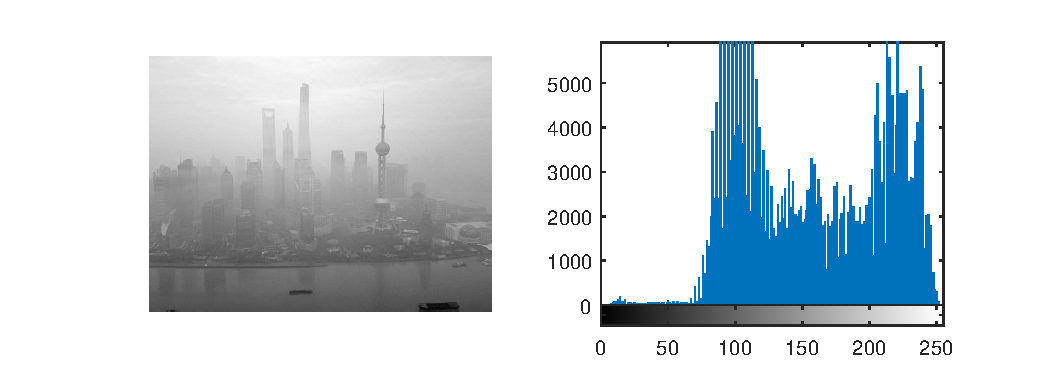
\includegraphics[totalheight=60mm]{./figures/ssr2.eps}
				\caption{SSR增强算法\label{SSR}}
			\end{figure}

从上图中可见,图2.4增强效果好,突出了图像细节,符合人眼感官。从图2.4的灰度直方图中可见,图中形状和图2.1中的灰度直方图相似,对比度加强,即同样被更加适当的“拉伸”了。
	\chapter{DWT-SVD增强算法}
		\section{奇异值分解算法}奇异值分解最初是由差分几何形成的,希望通过它所作用的两个空间的独立正交变换来确定真正的双线性形式是否可以与另一个形式相等。 Eugenio Beltrami和Camille Jordan分别在1873年和1874年分别发现了双线性形式的奇异值(用矩阵表示)形成了正交替换下双线性形式的一组完整的不变量。詹姆斯约瑟夫西尔维斯特在1889年也得到了实数矩阵的奇异值分解。西尔维斯特将奇异值称为矩阵$A$的正规乘子。第四位独立发现奇异值分解的数学家是1915年的Autonne,他通过极坐标分解到达它。矩阵和复矩阵的奇异值分解的第一个证乎是Carl Eckart和Gale Young于1936年提出的,他们将看作奇异值是Hermitian矩阵主轴变换的推广。1907年,艾哈德施密特为整数算子定义了一个奇异值的类比。似乎他并不知道有限矩阵奇异值的并行工作。计算SVD的实用方法可以追溯到1954年,1955年和1958年Hestenes 。类似于Jacobi特征值算法,它使用平面旋转或Givens旋转。然而,这些被Gene Golub和William Kahan于1965年发表的方法取代,使用Householder变换或反射。 1970年,Golub和Christian Reinsch 发表了Golub / Kahan算法的一个变体,该算法仍然是今天最常用的算法。

SVD定理的几何意义:对于每个线性映射$T:K^n→K^m$,可以找到$Kn$和$Km$的正交基,使得$T$将$Kn$的第$i$个基矢量映射到非负倍$Km$的第$i$个基矢量,并令剩余基矢量为零。

SVD是最小二乘意义下的最优矩阵分解,它将最大信号能量尽可能地分解为尽可能少的系数。奇异值分解(Singular Value Decomposition, SVD)是一种稳定而有效的方法,将系统分解为一组线性无关的分量,每个分量都对系统有一定程度上的贡献。奇异值分解是数值分析中用于对角化矩阵的数值技术。由于SVD具有无穷无尽的优点,如压缩中,在两个独特的子空间数据和噪声子空间的基础上处理图像的能力,所以SVD是一种有吸引力的图像处理代数变换,它通常用于噪声过滤,也被用于水印应用。这些应用程序中的每一个都利用了SVD的关键属性。奇异值分解是鲁棒可靠的正交矩阵分解方法,这是由于其概念和稳定性原因在信号处理领域越来越流行。本文主要介绍奇异值在图像增强的的应用。以下介绍奇异值分解的数学表达。
			\subsection{奇异值分解的数学表达}在线性代数中,SVD是矩阵实数或复数矩阵的分解,类似于使用特征向量的基础的对称或厄密特矩阵的数量化。 SVD是将系统分解为一组线性独立分量的稳定且有效的方法,具有$N \leq M$的尺寸为$M×N$的数字图像$X$可以通过其如下的SVD来表示;
\begin{equation}	\left[ X \right] _{N×M}=\left[ U \right] _{M×M} \left[ S \right] _{M×N} \left[ V \right] ^T_{N×N}	\end{equation}			
\[ U=[u_1,u_2....u_m],	V=[v_1,v_2....v_n] \]
\[
S
=\begin{bmatrix}
s_1  &  0  & \cdots\ &0\\
0  &  s_2  & \cdots\ & 0\\
 \vdots   & \vdots & \ddots  & \vdots  \\
 0 & 0  & \cdots\ & s_n\\
\end{bmatrix}
\]

其中$U$是$M×M$的正交矩阵,$V$是$N×N$的正交矩阵,$S$是$M×N$的矩阵,并且对角元素$s_i$是矩阵$X$的奇异值,下标$T$表示矩阵的转置。正交矩阵$U$的列被称为左奇异向量(Left Singular Vector, LSV),正交矩阵$V$的列被称为右奇异向量(Right Singular Vector, RSV)。$X$的左奇异向量是$XX^T$的特征向量,$X$的右奇异向量是$X^TX$的特征向量。每个奇异值(singular value,SV)指定图像层的亮度,而相应的奇异向量指定图像的几何形状。 U和V是正交矩阵(每列的平方和是独立的,且每个列互不相关),$S$是奇异值递减的对角矩阵。%每个特征图像的奇异值就是它的2-范数。因为SVD使最大奇异值最大化,所以第一特征图像是占最大量的方差 - 协方差结构的模式

		小波变换-数字图像处理p320
		\section{小波变换理论}在数值分析和功能分析中,离散小波变换(Discrete Wavelet Transform, DWT)是对任何小波进行离散采样的小波变换。 。小波变换的基本思想是可变窗口的平移和伸缩的基本思想。Haar基是一种最简单的小波基,具有不连续性的特点。小波变换能自动调节频率窗口和时间窗口并能使频域和时域同时进行局部变换,这一特点是小波变换优于傅里叶变换的地方。小波的特点有:长度有限,均值为零。小波变换能够使用伸缩和平移的特性从多个角度细化目标函数。

与小波变换有关的第一个文献是Haar小波。 它是1909年由数学家Alfrd Haar提出的。然而,小波的概念当时并不存在。 直到1981年,这个概念才由地球物理学家让·莫雷特提出。 之后,Morlet和物理学家Alex Grossman在1984年发明了小波项。在1985年之前,Haar小波是人们唯一知道的正交小波。 许多研究人员甚至认为除了Haar小波之外没有正交小波。 此后,数学家Yves Meyer于1985年构造了第二个正交小波Meyer小波。随着越来越多的学者加入这一领域,第一次国际会议于1987年在法国举行。1988年,Stephane Mallat和Meyer提出了多重解决的概念。 同年,Ingrid Daubechies发现了一种构造紧支撑正交小波的系统方法。 1989年,Mallat提出了快速小波变换。 随着这种快速算法的出现,小波变换在信号处理领域有很多应用。
			\subsection{离散小波变换}二维离散小波变换是连续信号离散化后的小波变换,可以用来分析诸如图像的二维离散信号,并在图像压缩领域,数字水印领域,图像融合领域皆有所应用。本文着重强调其在图像增强上的应用。DWT示意图图如下所示:
				\begin{figure}[!ht]\centering
					\includegraphics[totalheight=40mm,width=160mm]{./figures/DWT.jpg}
					\caption{DWT二级小波变换分解图\label{DWT}}	
				\end{figure}		

其中,$L$是高低滤波器,$H$是高通滤波器。原始图像经过以及分解后会得到$LL_1$、$HL_1$、$LH_1$、$HH_1$四个子带,子带即一幅图像被分解为一组频带受限的分量,并且子带可以重组在一个构成无误差的原始图像。$LL_1$是水平及垂直方向上的低频子带,$LH_1$是水平方向上低频并且垂直方向上高频的子带,$HL_1$是水平方向上高频并且垂直方向上低频的子带,$HH_1$是水平及垂直方向上都高频的子带。而$LL_2$、$HL_2$、$LH_2$、$HH_2$是子带$LL_1$再次进行一次DWT运算的子带。现在以第一次小波分解为例,进行演示。
				\begin{figure}[ht]
					\begin{minipage}{0.48\linewidth}
						\centerline{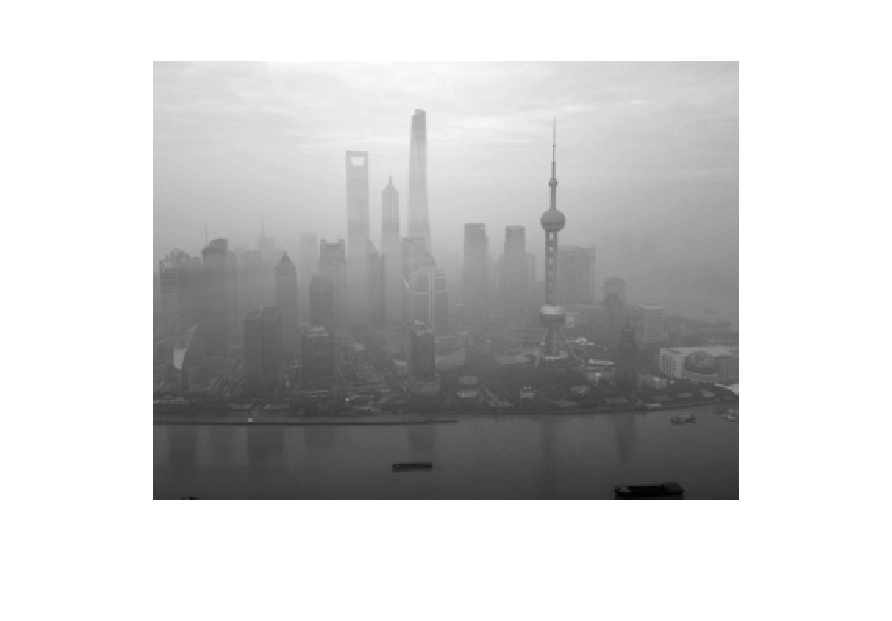
\includegraphics[width=1\textwidth]{./figures/LL.eps}}
						\centerline{LL}
					\end{minipage}
					\qquad
					\begin{minipage}{0.48\linewidth}
						\centerline{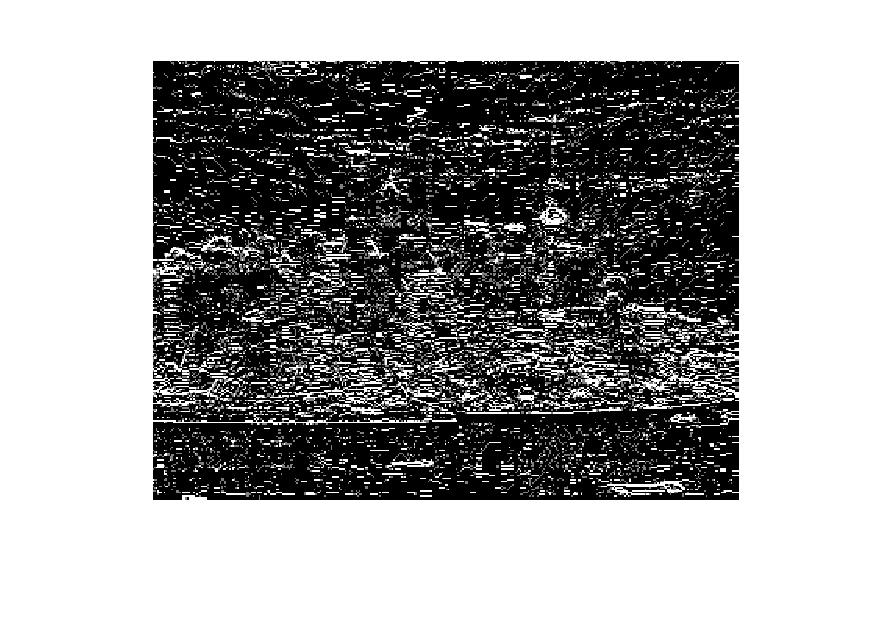
\includegraphics[width=1\textwidth]{./figures/HL.eps}}
						\centerline{HL}
					\end{minipage}

					\begin{minipage}{0.48\linewidth}
						\centerline{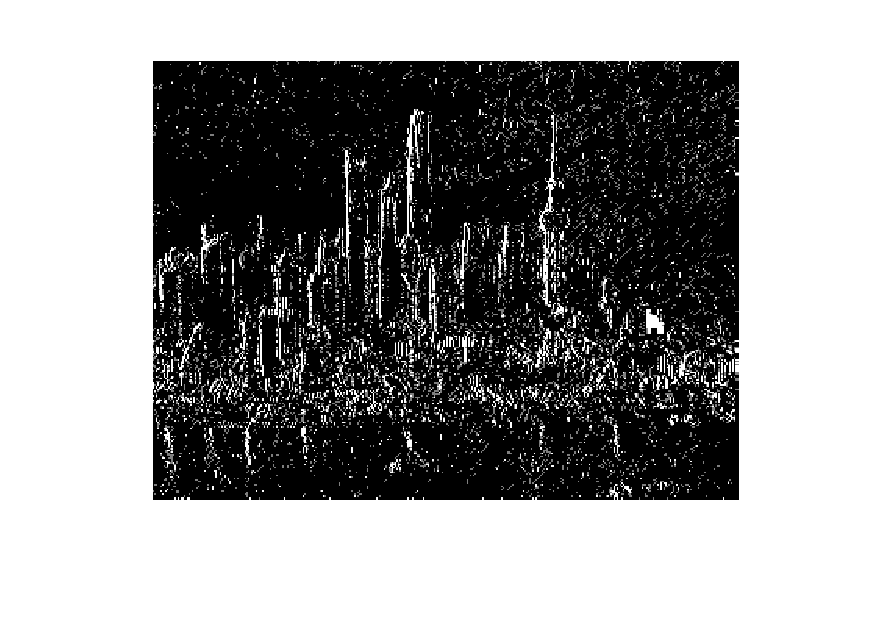
\includegraphics[width=1\textwidth]{./figures/LH.eps}}
						\centerline{LH}
					\end{minipage}
					\qquad
					\begin{minipage}{0.48\linewidth}
						\centerline{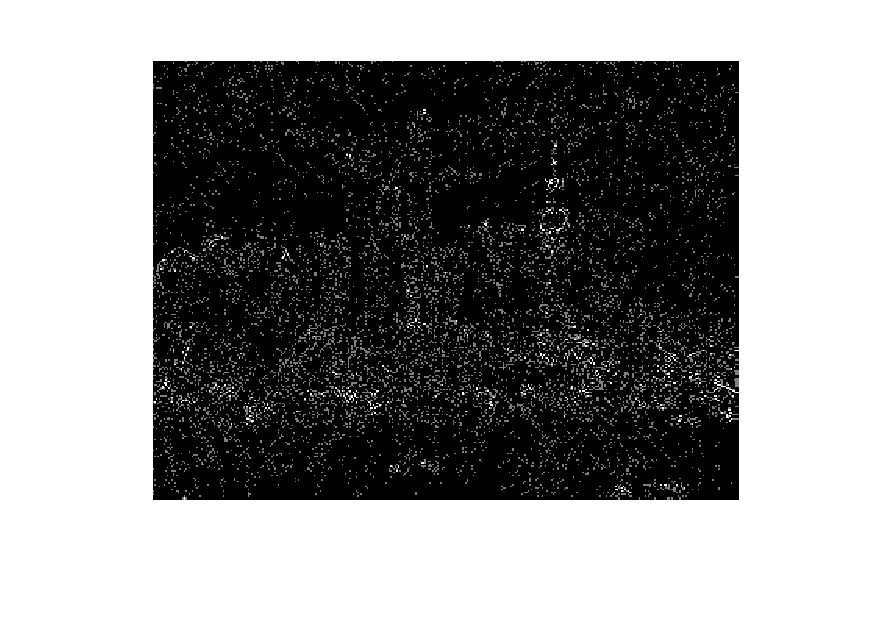
\includegraphics[width=1\textwidth]{./figures/HH.eps}}
						\centerline{HH}
					\end{minipage}
					\caption{DWT示例\label{DWT}}
				\end{figure}

这里图像的频率指的是图像中灰度变化剧烈强度,是灰度平面上的梯度。图像中的高频分量,指的是图像强度(亮度、灰度)变化剧烈的地方,即边缘(轮廓)以及细节特征。图像中的低频分量,指的是图像强度(亮度、灰度)变换平缓的地方,即大片色块的地方。从图$3.2$中可以看出子带$LL$中包含了原始图像的大部分信息,子带$HL$中主要包含了原始图像的水平方向的轮廓信息,子带$HL$中主要包含了原始图像的垂直方向的轮廓信息,子带$HH$中主要包含了原始图像的轮廓信息及其噪声。以下将展示离散小波变换在保留图像轮廓中的应用。

图$3.3$是子带$HL$、$LH$、$HH$与一个横列分别与子带$LL$相同的零矩阵(即规模相同的全黑矩阵)进行离散小波反变换(IDWT)的结果图,从中可以看出离散小波反变换可以将子带$HL$、$LH$、$HH$还原成一幅保留原始图像大致轮廓的轮廓图。并且用离散小波反变换将子带$LL$、$HL$、$LH$、$HH$还原而成的图像将于原始图像一致,不会有数据丢失。
			\begin{figure}[!ht]\centering
				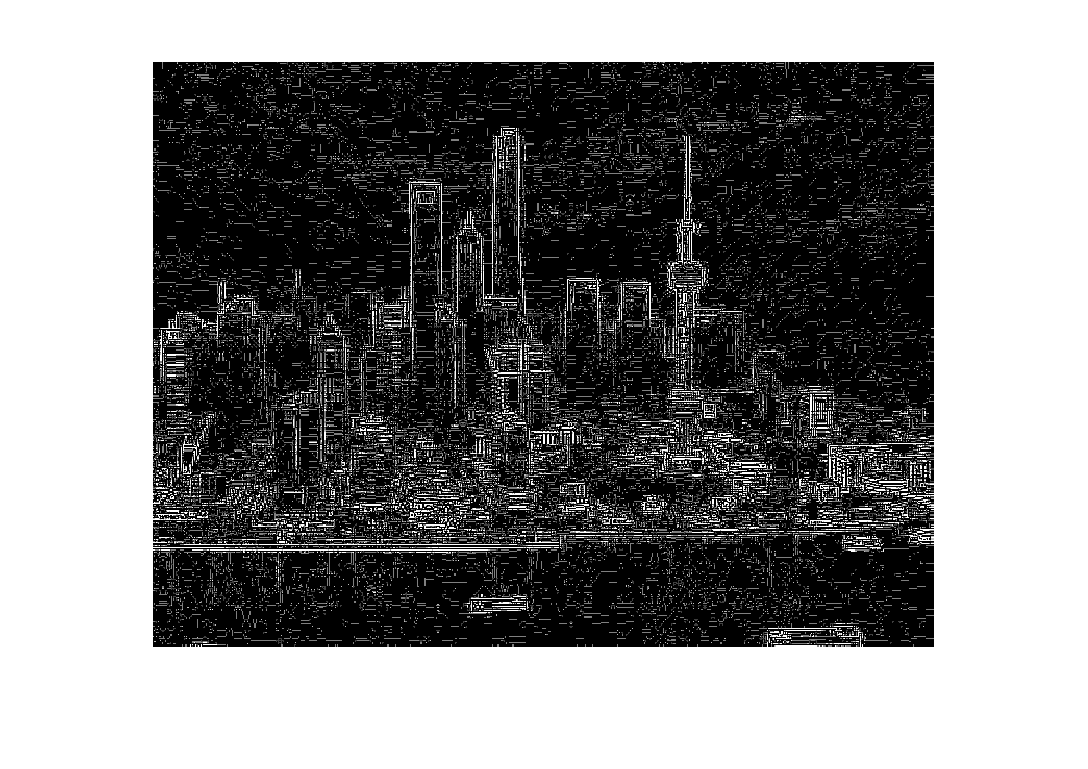
\includegraphics[totalheight=60mm]{./figures/replaceImageLL.eps}
				\caption{DWT在保留轮廓中的应用\label{DWT}}
			\end{figure}


	\section{DWT-SVD算法}本文提出的基于DWT-SVD算法的航空图像增强分成为两个部分,第一个部分是使用奇异值分解获得原始图像的奇异值矩阵,改变奇异值矩阵中的数值将会直接影响到图像的亮度并且其余信息保持不变\cite{improved...}。第二部分,是使用直方图均衡,使目标图像的对比度增强。第三部分是使用离散小波变换对原始图像进行处理以保留原始图像的主要轮廓和图像细节,以便进行还原是最终图像有较好的对比度和图像细节。

首先,对输入的灰度航空图像‘$A$’进行直方图均衡处理生成‘$A^*$’,在得到‘$A^*$’后对图像‘$A$’和图像‘$A^*$’进行离散小波变换,分别得到子带$LL$、$HL$、$LH$、$HH$和子带$LL^*$、$HL^*$、$LH^*$、$HH^*$。第二部分别对子带$LL$和$LL^*$进行奇异值分解得到$U_{LL}$、$S_{LL}$、$V_{LL}$和$U_ {LL^*}$、$S_{LL^*}$、$V_{LL^*}$。然后通过下式计算两个奇异值矩阵的相关系数:
\begin{equation}     \xi = \frac{max \left( S_{LL^*} \right) }{ max \left( S_{LL} \right) }    \end{equation}

其中,$S_{LL}$是原始图像$A$的低频系数奇异矩阵,$S_{LL^*}$是原始图像经过直方图均衡化后得到的图像$A^*$的低频系数奇异矩阵。
\begin{equation}     \bar{S}_{LL} = \xi S_{LL}    \end{equation}
\begin{equation}     \bar{LL} =  U_{LL} \bar{S}_{LL} V_{LL} \end{equation}

式$3.2$和式子$3.3$的效果是将使直方图均衡化后的图像‘$A^*$’(或是包含了‘$A^*$’大部分信息的子带$LL^*$)所具有的使图像对比度增强的性质赋予了子带$LL$产生新的子带$\bar{LL}$。式$3.4$中的$\bar{LL}$为低频系数矩阵$S_{LL}$经过奇异值矩阵的相关系数$\xi$增强后再经过奇异值分解公式得到的结果。然后在对进行$\bar{LL}$、$HL$、$LH$、$HH$进行离散小波变换:
\begin{equation}     \bar{A} = IDWT(\bar{LL},HL,LH,HH)    \end{equation}

由于直方图均衡能使图像对比度增强,视觉效果好。离散小波变换能使图像保留原有的轮廓信息和图像细节。然后通过奇异值分解“连接”这两个算法。这样使得了最终图像$\bar{A}$具有更好的视觉效果和更多的轮廓信息,以达到图像增强的效果。以下展示DWT-SVD的算法流程图:
			\begin{figure}[!ht]\centering
				\includegraphics[]{./figures/flowChatOfDWTSVD.jpg}
				\caption{DWT-SVD的算法流程图\label{DWT}}
			\end{figure}

以下将展示原始图像经过DWT-SVD算法增强后的结果:
				\begin{figure}[ht]
					\begin{minipage}{0.48\linewidth}
						\centerline{\includegraphics[width=1\textwidth]{./figures/originalImage.eps}}
						\centerline{原始图像}
					\end{minipage}
					\qquad
					\begin{minipage}{0.48\linewidth}
						\centerline{\includegraphics[width=1\textwidth]{./figures/DWTSVDExample.eps}}
						\centerline{DWT-SVD增强处理}
					\end{minipage}
					\caption{DWT-SVD示例\label{DWT}}
				\end{figure}

可以从图





%下一步:LL=0矩阵 然后融合
%dwt:轮廓保留  
%svd:内容增强

		
	\chapter{实验结果及指标分析}
		\section{图像评价的客观指标}对图像质量的客观指标分为主观评价和客观评价。主观评价即这幅图片给人的视觉效果较好,使大多数人的主观感受感到舒适。而客观评价也是必不可少的,是一个算法是否有效的重要依据。但是由于不同种类的图像具有不同的特性,并且由于工程任务的目标的不同,即使是对同一种类的图像也可能提出不同的要求,因此很难有一种客观评价指标是适用于大多数图片的。本文使用图像灰度均值,图像灰度标准差,图像信息熵以及图像灰度直方图作为图像客观评价指标。将多种指标放在一起进行比较。以证明本文方法的有效性以及与其他方法的异同。
			\subsection{灰度均值}图像灰度均值表示图像的整体亮度,是一个宏观指标,是图像亮度给人的第一视觉感觉的客观反映。当图像均值一直在灰度值为128的地方小范围波动时,大多数情况下图像具有较好的视觉效果,但是例如当图像在雾天拍摄时所得的图像,不符合上述规律。图像灰度均值的计算公式如下:
\begin{equation}	u= \frac{1}{WH} \sum \sum R(x,y) 	\end{equation}	
	
此处,$WH$为图像尺寸的乘积,即宽度$W$与$H$相乘。

			\subsection{灰度标准差}图像标准差反映了图像像素灰度值与均值的离散程度,标准差越大说明图像各个像素点灰度值之间的离散化程度越高,其数学表达式为:
\begin{equation}	 	\sigma =  \sqrt{ \frac{1}{WH} \sum \sum R(x,y-u)^2}	\end{equation}

图像的灰度值标准差表示图像的的亮暗范围,标准差数值越大即表明图片所显示的亮暗范围越大。
			\subsection{图像信息熵}图像信息熵是一种统计形式,用以对图像中的平均信息量的大小进行量化。信息熵即衡量信息量的指标,信息熵满足三条性质:单调性即发生概率越高的事件所携带的信息熵越低,非负性即信息熵不能为复数和累加性。简单的说,就是信息熵是按平均概率发生一个事件观察者能得到的信息量的大小。在数学上,信息熵就是信息量的期望。图像信息熵分为一维灰度信息熵和二维灰度信息熵。其中一维灰度信息熵无法反应信息在图像二维空间上分布的特征。因此本文的图像信息熵特指二维灰度信息熵。图像信息熵的大小和图像所单位面积内包含的信息量的大小成正相关,即图像信息熵越大,图像单位面积所包含的信息量的大小越大。图像信息熵的数学表达为:
\begin{equation}	 	P = - \sum p_iln(p_i)		\end{equation}

其中,求和的范围为从灰度值的最低值到灰度值的最高值,$p_i$代表每个灰度级的概率。

		\section{实验结果}本问提出的算法是对航空图像进行增强处理,因此要充分考虑到恶劣状况对航空图像的影响。因此我们挑选两类图片进行实验,分别用直方图均衡、SSR算法和DWT—SVD算法对他们进行处理,并对结果进行分析和比较。
			\subsection{第一组实验}第一组实验对具有整体低对比度,整体偏白的特征的图片进行增强处理,即对在雾天条件下拍摄的图片进行处理。

				\begin{figure}[!ht]
					\begin{minipage}{0.48\linewidth}
						\centerline{\includegraphics[width=1\textwidth]{./figures/originalImage.eps}}
						\centerline{原图像}
					\end{minipage}
					\qquad
					\begin{minipage}{0.48\linewidth}
						\centerline{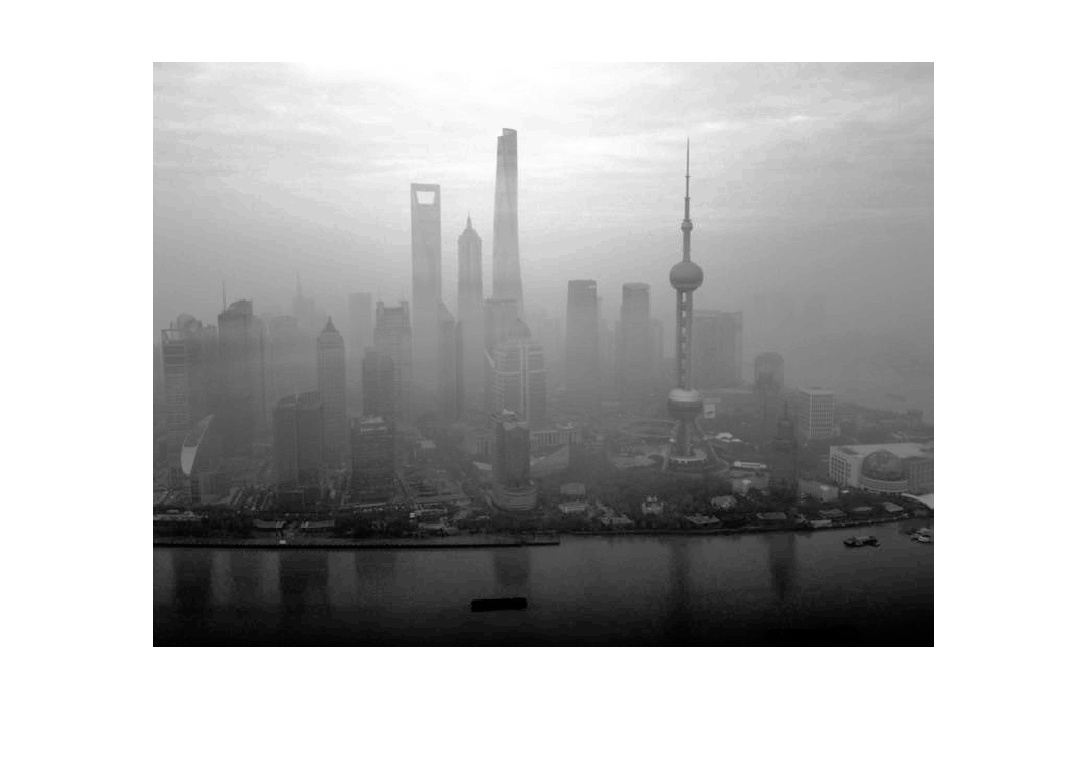
\includegraphics[width=1\textwidth]{./figures/HE11.eps}}
						\centerline{直方图均衡增强后图像}
					\end{minipage}

					\begin{minipage}{0.48\linewidth}
						\centerline{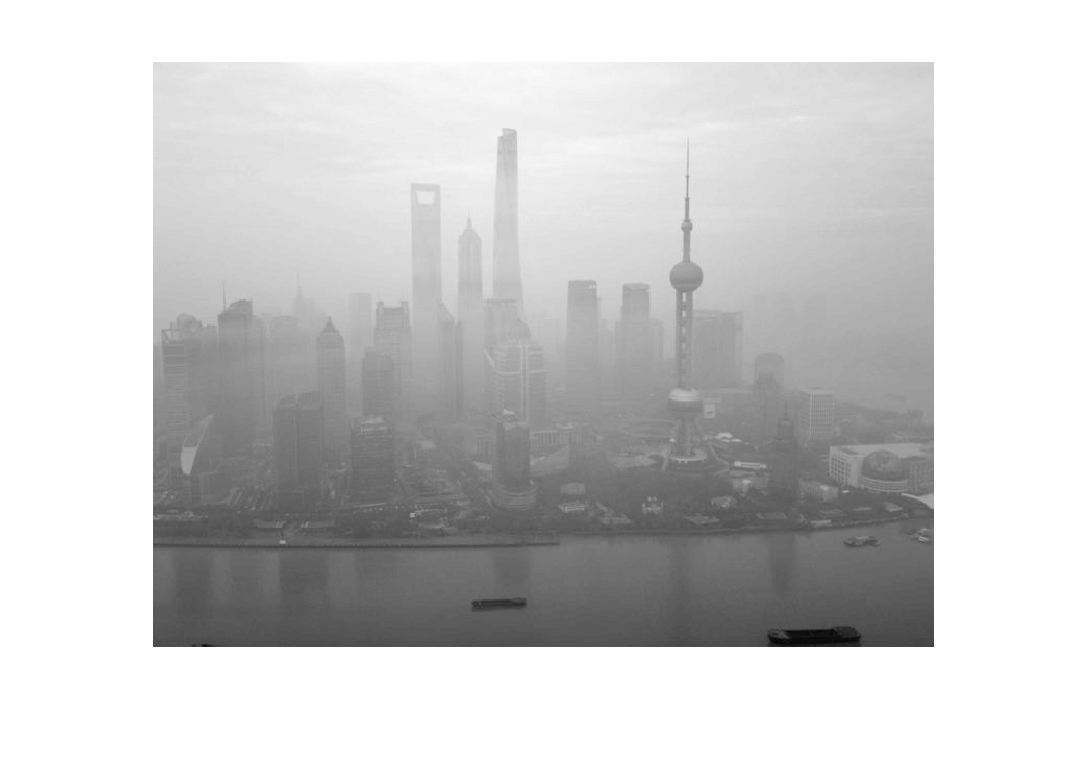
\includegraphics[width=1\textwidth]{./figures/ssr11.eps}}
						\centerline{SSR算法增强后图像}
					\end{minipage}
					\qquad
					\begin{minipage}{0.48\linewidth}
						\centerline{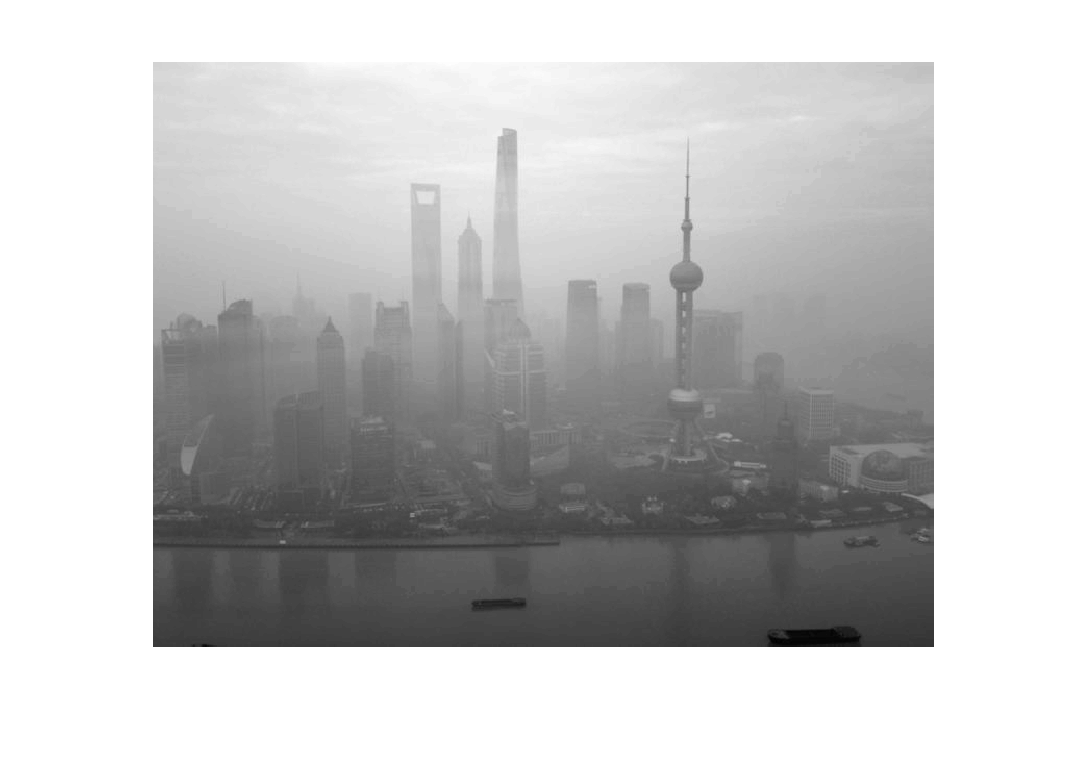
\includegraphics[width=1\textwidth]{./figures/DWTSVD11.eps}}
						\centerline{DWT-SVD算法增强后图像}
					\end{minipage}
					\caption{3种算法结果图比较\label{ }}
				\end{figure}

主观上分析,可以从图$4.1$中看出原图像的特点为:图像整体模糊不清,近景的物体依稀可见有一条和几条船,远景的物体是一些看不清楚但是可以逻辑判断出的建筑物,但是城市中的道路和建筑轮廓人眼难以辨认。直方图均衡算法增强后的图像整体视觉效果更好,并且城市中的道路和建筑轮廓清晰可辨,但是存在过增强的缺点。例如此图片右下角呈现出全黑的局部图象,但是原图中可以看见有一只小船。单尺度Retinex算法增强后的图像右下角有船只即没有展现出过增强的迹象,也实现了去雾的效果,但是部分细节不如直方图均衡算法的结果清晰。总体而言,单尺度Retinex算法的效果比直方图均衡的效果在雾天航空图像上来的好。而DWT-SVD增强算法的主观效果整体相差不大,但在局部,例如城市中的建筑轮廓与背景比较,DWT-SVD算法的结果更加清晰,更好的改善视觉效果。

%    \begin{table}  
%    \caption{设置表格总长}  
%    \begin{tabular*}{12cm}{lll}  
%    \hline  
%    算法&均值&标准差&信息熵\\
%    \hline  
%    原始图像& 140.48& 21.35&6.07\\ 
%    直方图均衡& 129.61& 73.47&6.04\\  
%	SSR算法& 163.69& 53.24&7.19\\
%	DWT-SVD算法& 147.93& 58.64&7.47\\
%    \hline  
%    \end{tabular*}  
%    \end{table}  
从客观指标来看,可以从表格中看出,四幅图片的均值都偏高图像整体显示出白色,增强算法增强后的结果图的标准差数值大小普遍偏大,在一定程度上说明图像质量较好,而在图像信息熵方面增强算法增强后的图像的数值比原图像的数值大,也说明这三种的算法的有效的增加了原图像的信息量,其中DWT-SVD算法最为出众,其次是SSR算法。
			\subsection{第一组实验}第二组实验对具有整体对比度偏低,其中部分地方偏白的特点,拍摄场景为在薄雾天气,阳光较为强烈的条件下拍摄。

				\begin{figure}[!ht]
					\begin{minipage}{0.48\linewidth}
						\centerline{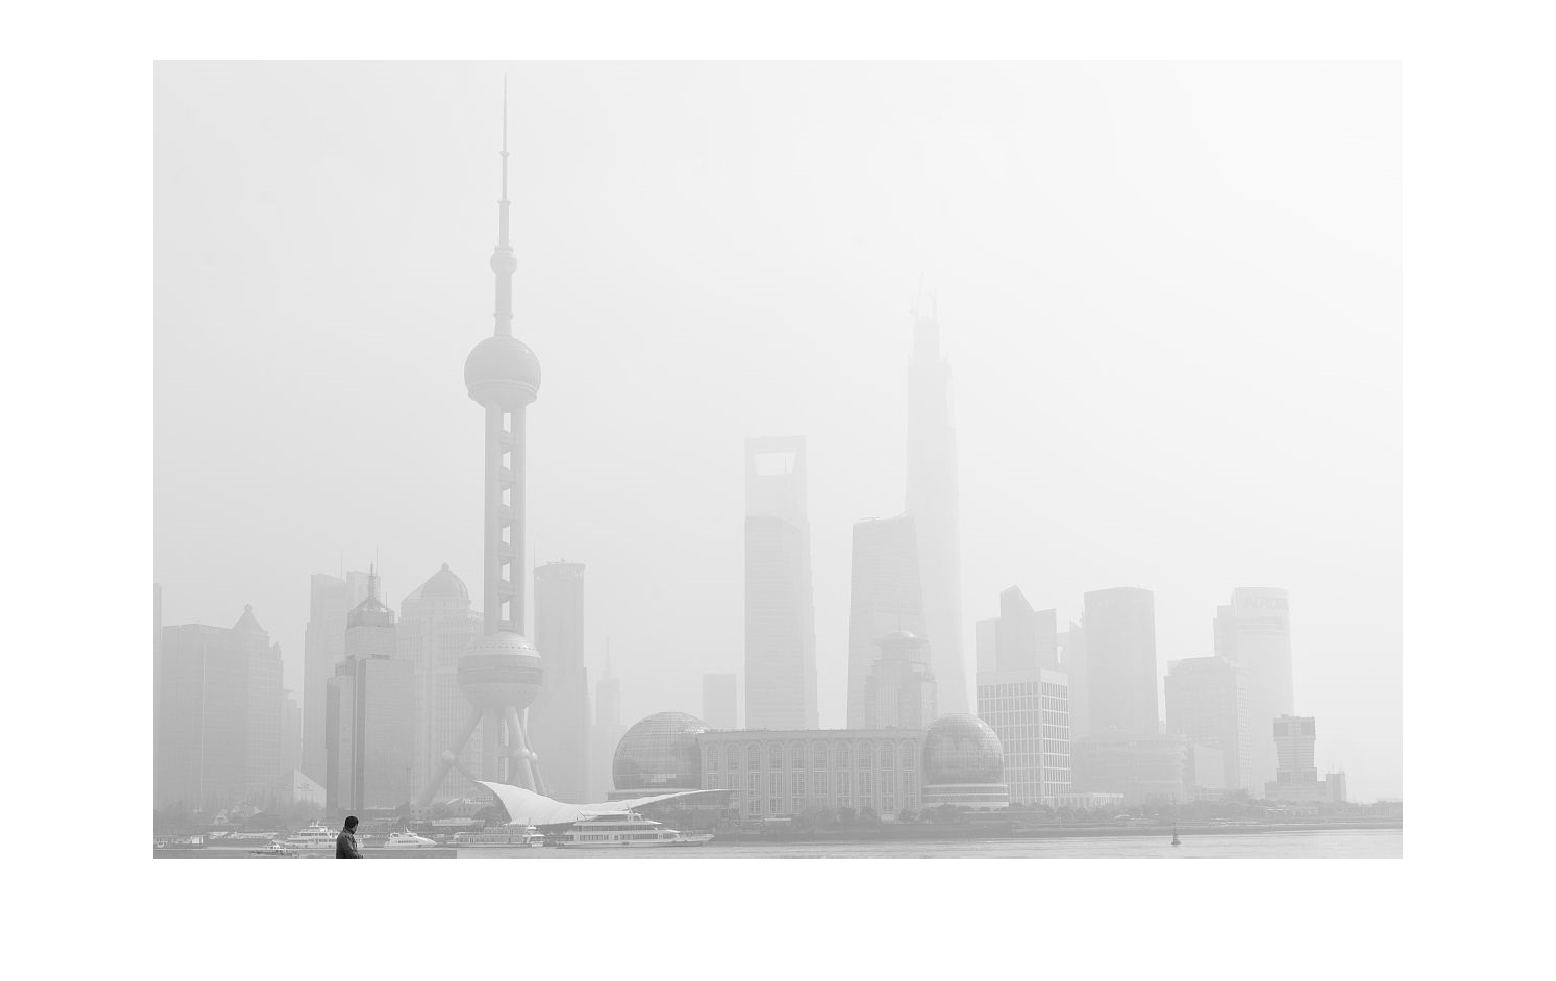
\includegraphics[width=1\textwidth]{./figures/originalImage16.eps}}
						\centerline{原图像}
					\end{minipage}
					\qquad
					\begin{minipage}{0.48\linewidth}
						\centerline{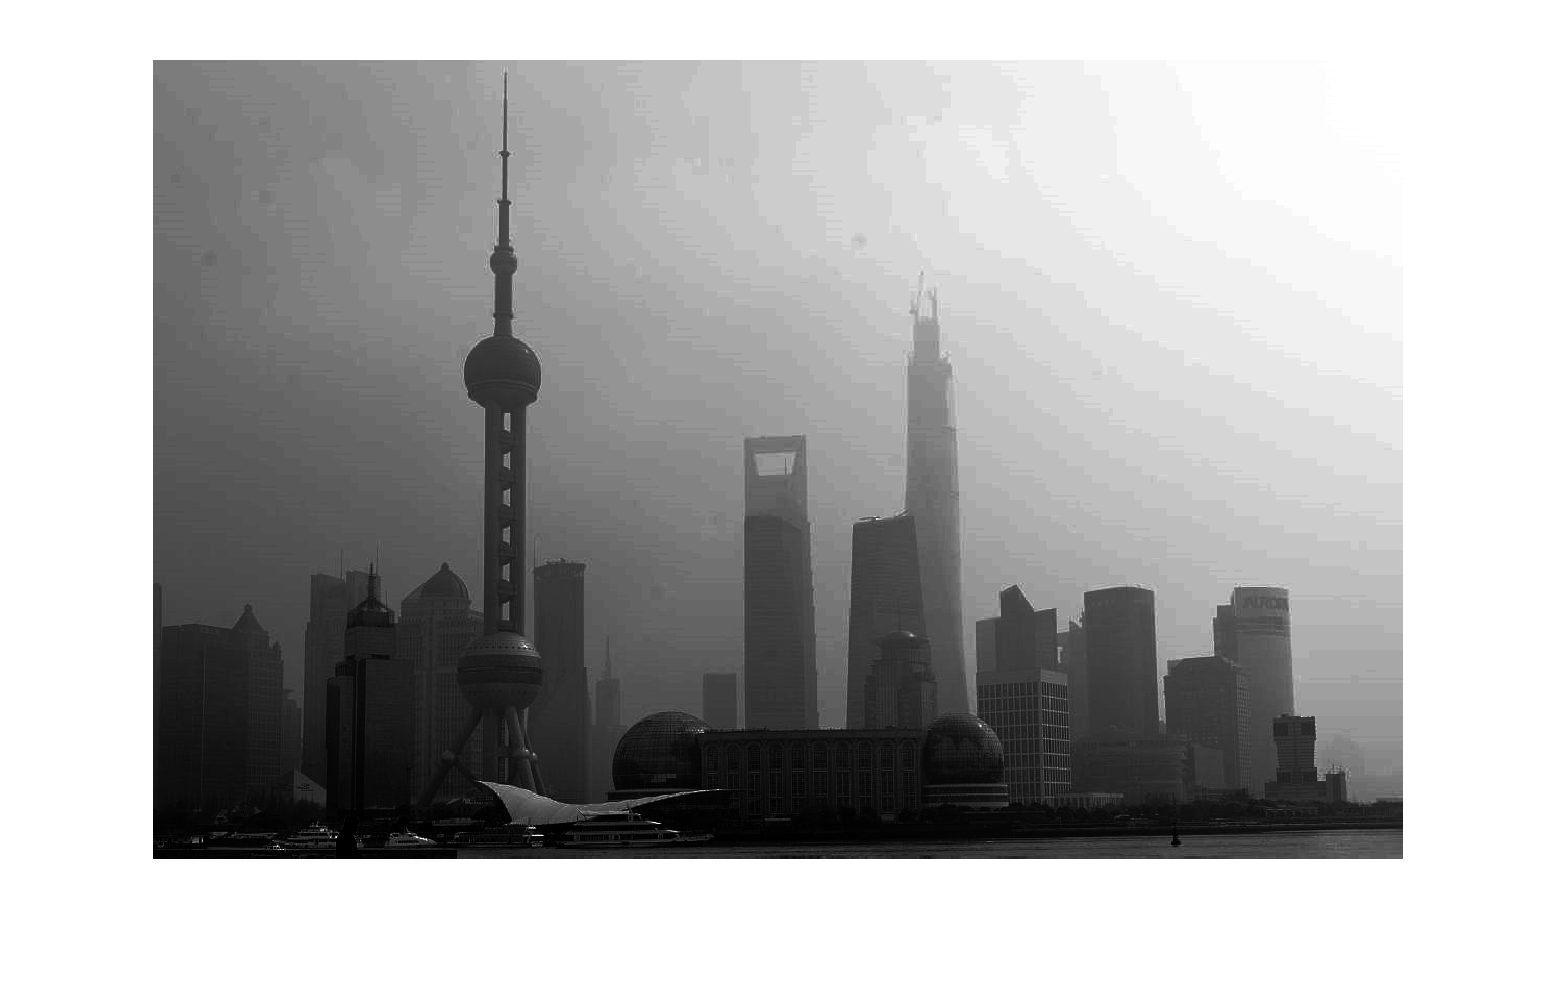
\includegraphics[width=1\textwidth]{./figures/HE16.eps}}
						\centerline{直方图均衡增强后图像}
					\end{minipage}

					\begin{minipage}{0.48\linewidth}
						\centerline{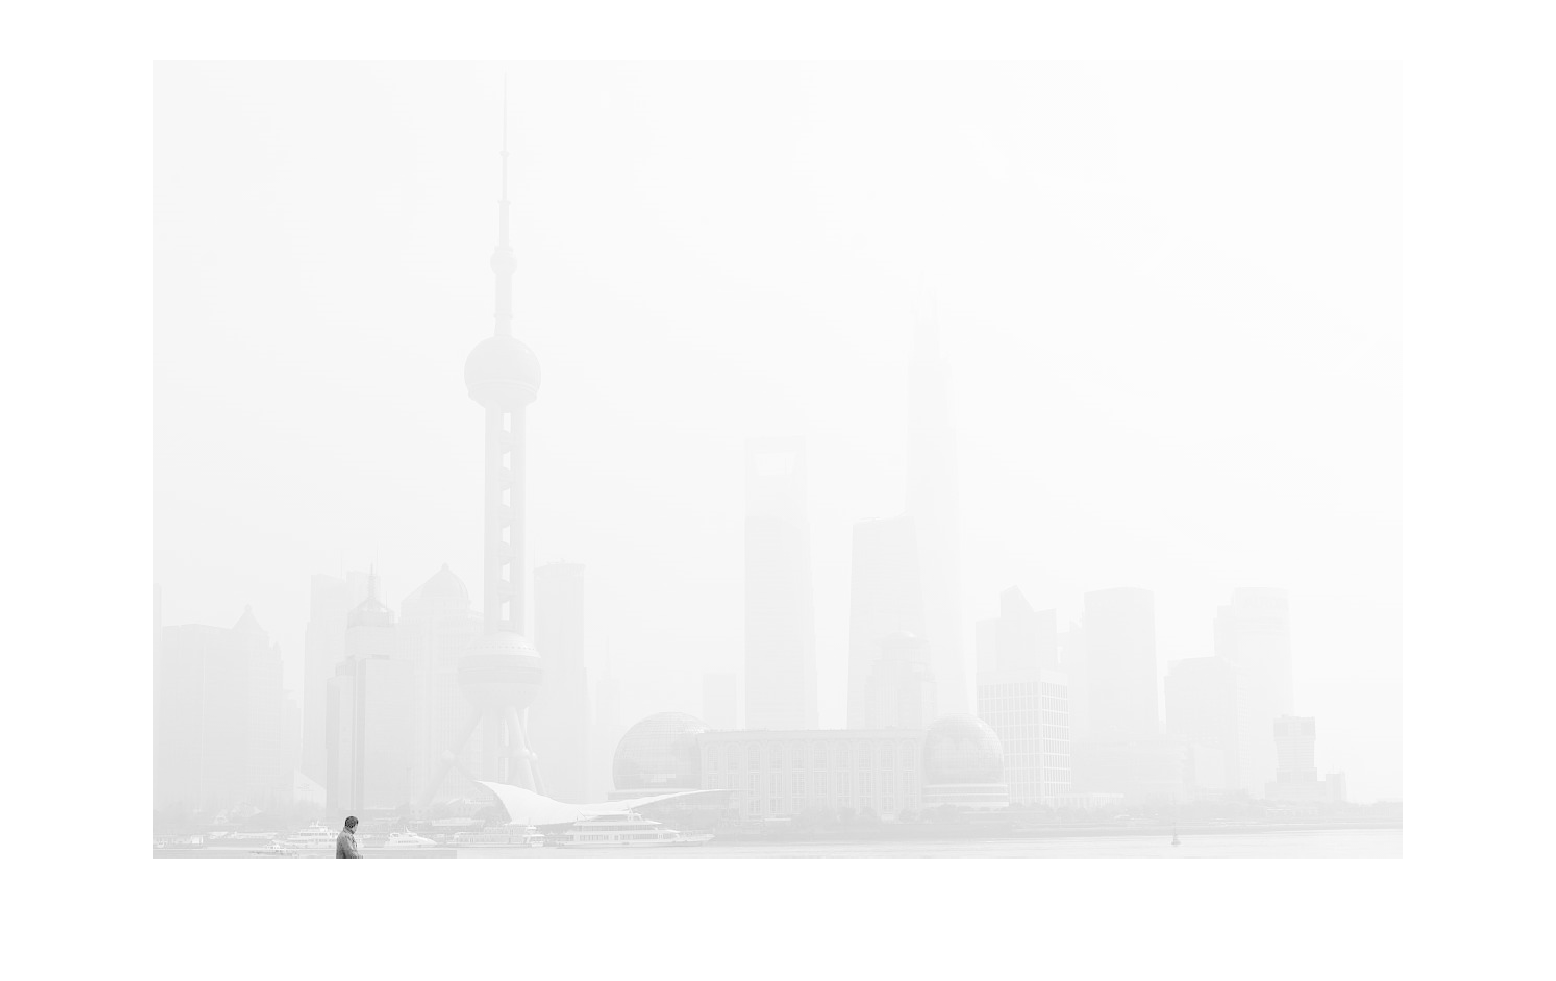
\includegraphics[width=1\textwidth]{./figures/ssr16.eps}}
						\centerline{SSR算法增强后图像}
					\end{minipage}
					\qquad
					\begin{minipage}{0.48\linewidth}
						\centerline{\includegraphics[width=1\textwidth]{./figures/DWTSVD16.eps}}
						\centerline{DWT-SVD算法增强后图像}
					\end{minipage}
					\caption{3种算法结果图比较\label{ }}
				\end{figure}

图4.2中直方图均衡算法造成了多处地方细节丢失,但也有让观察者更清楚的看清楚建筑轮廓的优点,而SSR算法效果不理想整体偏白,看不清细节,图像效果不如原图,SSR算作作为一种经典的去雾算法在此种场景并不适用。DWT-SVD算法图像效果和原图相差不大,但是在此类图像上的整体效果显然优于直方图均衡和SSR算法增强后的结果。
	\chapter{结论}\label{chap:zongJie}航空图像一直是社会工作和工程项目中的研究热点,本文针对雾天拍摄得到的航空图像使用多种方法进行增强处理,针对同一种对象不同算法所得出的效果图和评价指标进行对比。并介绍了直方图均衡算法、Retinex算法和DWT-SVD算法在各个方面的优缺点。

本为从奇异值分解、离散小波变换理论出发,将两者与直方图均衡结合起来,实现了航空图像自适应的功能,结合了离散小波算法和直方图均衡的优点,并削减了它们的缺点。虽然在识别远处物体轮廓方面不如直方图均衡,但是在细节保留方面却远远的强与直方图均衡,因而能够达到一个整体效果相对好的增强图像。在去雾方面的效果与SSR算法相差不大,但是SSR算法在部分图像的增强效果甚至不如原始图像,因此本文算法在自适应方面优于SSR算法。但是在DWT-SVD算法无法对所有的雾天航空图像起到很好的增强效果,关于如何提高改算法,还有待研究













\end{document}




